%!TEX TS-program = xelatex
\documentclass[]{friggeri-cv}
\usepackage{afterpage}
\usepackage{hyperref}
\usepackage{color}
\usepackage{xcolor}
\usepackage{smartdiagram}

\usepackage{fontspec}
% if you want to add fontawesome package
% you need to compile the tex file with LuaLaTeX
% References:
%   http://texdoc.net/texmf-dist/doc/latex/fontawesome/fontawesome.pdf
%   https://www.ctan.org/tex-archive/fonts/fontawesome?lang=en
%\usepackage{fontawesome}
\usepackage{metalogo}
\usepackage{dtklogos}
\usepackage[utf8]{inputenc}
\usepackage{tikz}
\usetikzlibrary{mindmap,shadows}
\hypersetup{
    linkcolor=blue,
    filecolor=magenta,      
    urlcolor=cyan,
    pdftitle={CV of Aaron Schneider},
}

\smartdiagramset{
    bubble center node font = \footnotesize,
    bubble node font = \footnotesize,
    % specifies the minimum size of the bubble center node
    bubble center node size = 0.5cm,
    %  specifies the minimum size of the bubbles
    bubble node size = 0.5cm,
    % specifies which is the distance among the bubble center node and the other bubbles
    distance center/other bubbles = 0.3cm,
    % sets the distance from the text to the border of the bubble center node
    distance text center bubble = 0.5cm,
    % set center bubble color
    bubble center node color = pgray,
    % define the list of colors usable in the diagram
    set color list = {lightgray, materialcyan, orange, green, materialorange, materialteal, materialamber, materialindigo, materialgreen, materiallime},
    % sets the opacity at which the bubbles are shown
    bubble fill opacity = 0.6,
    % sets the opacity at which the bubble text is shown
    bubble text opacity = 0.5,
}

%\addbibresource{bibliography.bib}
\RequirePackage{xcolor}
\definecolor{pblue}{HTML}{0395DE}
\definecolor{pgray}{HTML}{6E6E6E}

\begin{document}
\header{\hspace{1.2cm}Aaron David}{ Schneider}{(Astro)physicist and software engineer}


% Fake text to add separator
\fcolorbox{white}{gray}{\parbox{\dimexpr\textwidth-2\fboxsep-2\fboxrule}{%
.....
}}

% In the aside, each new line forces a line break
\begin{aside}
  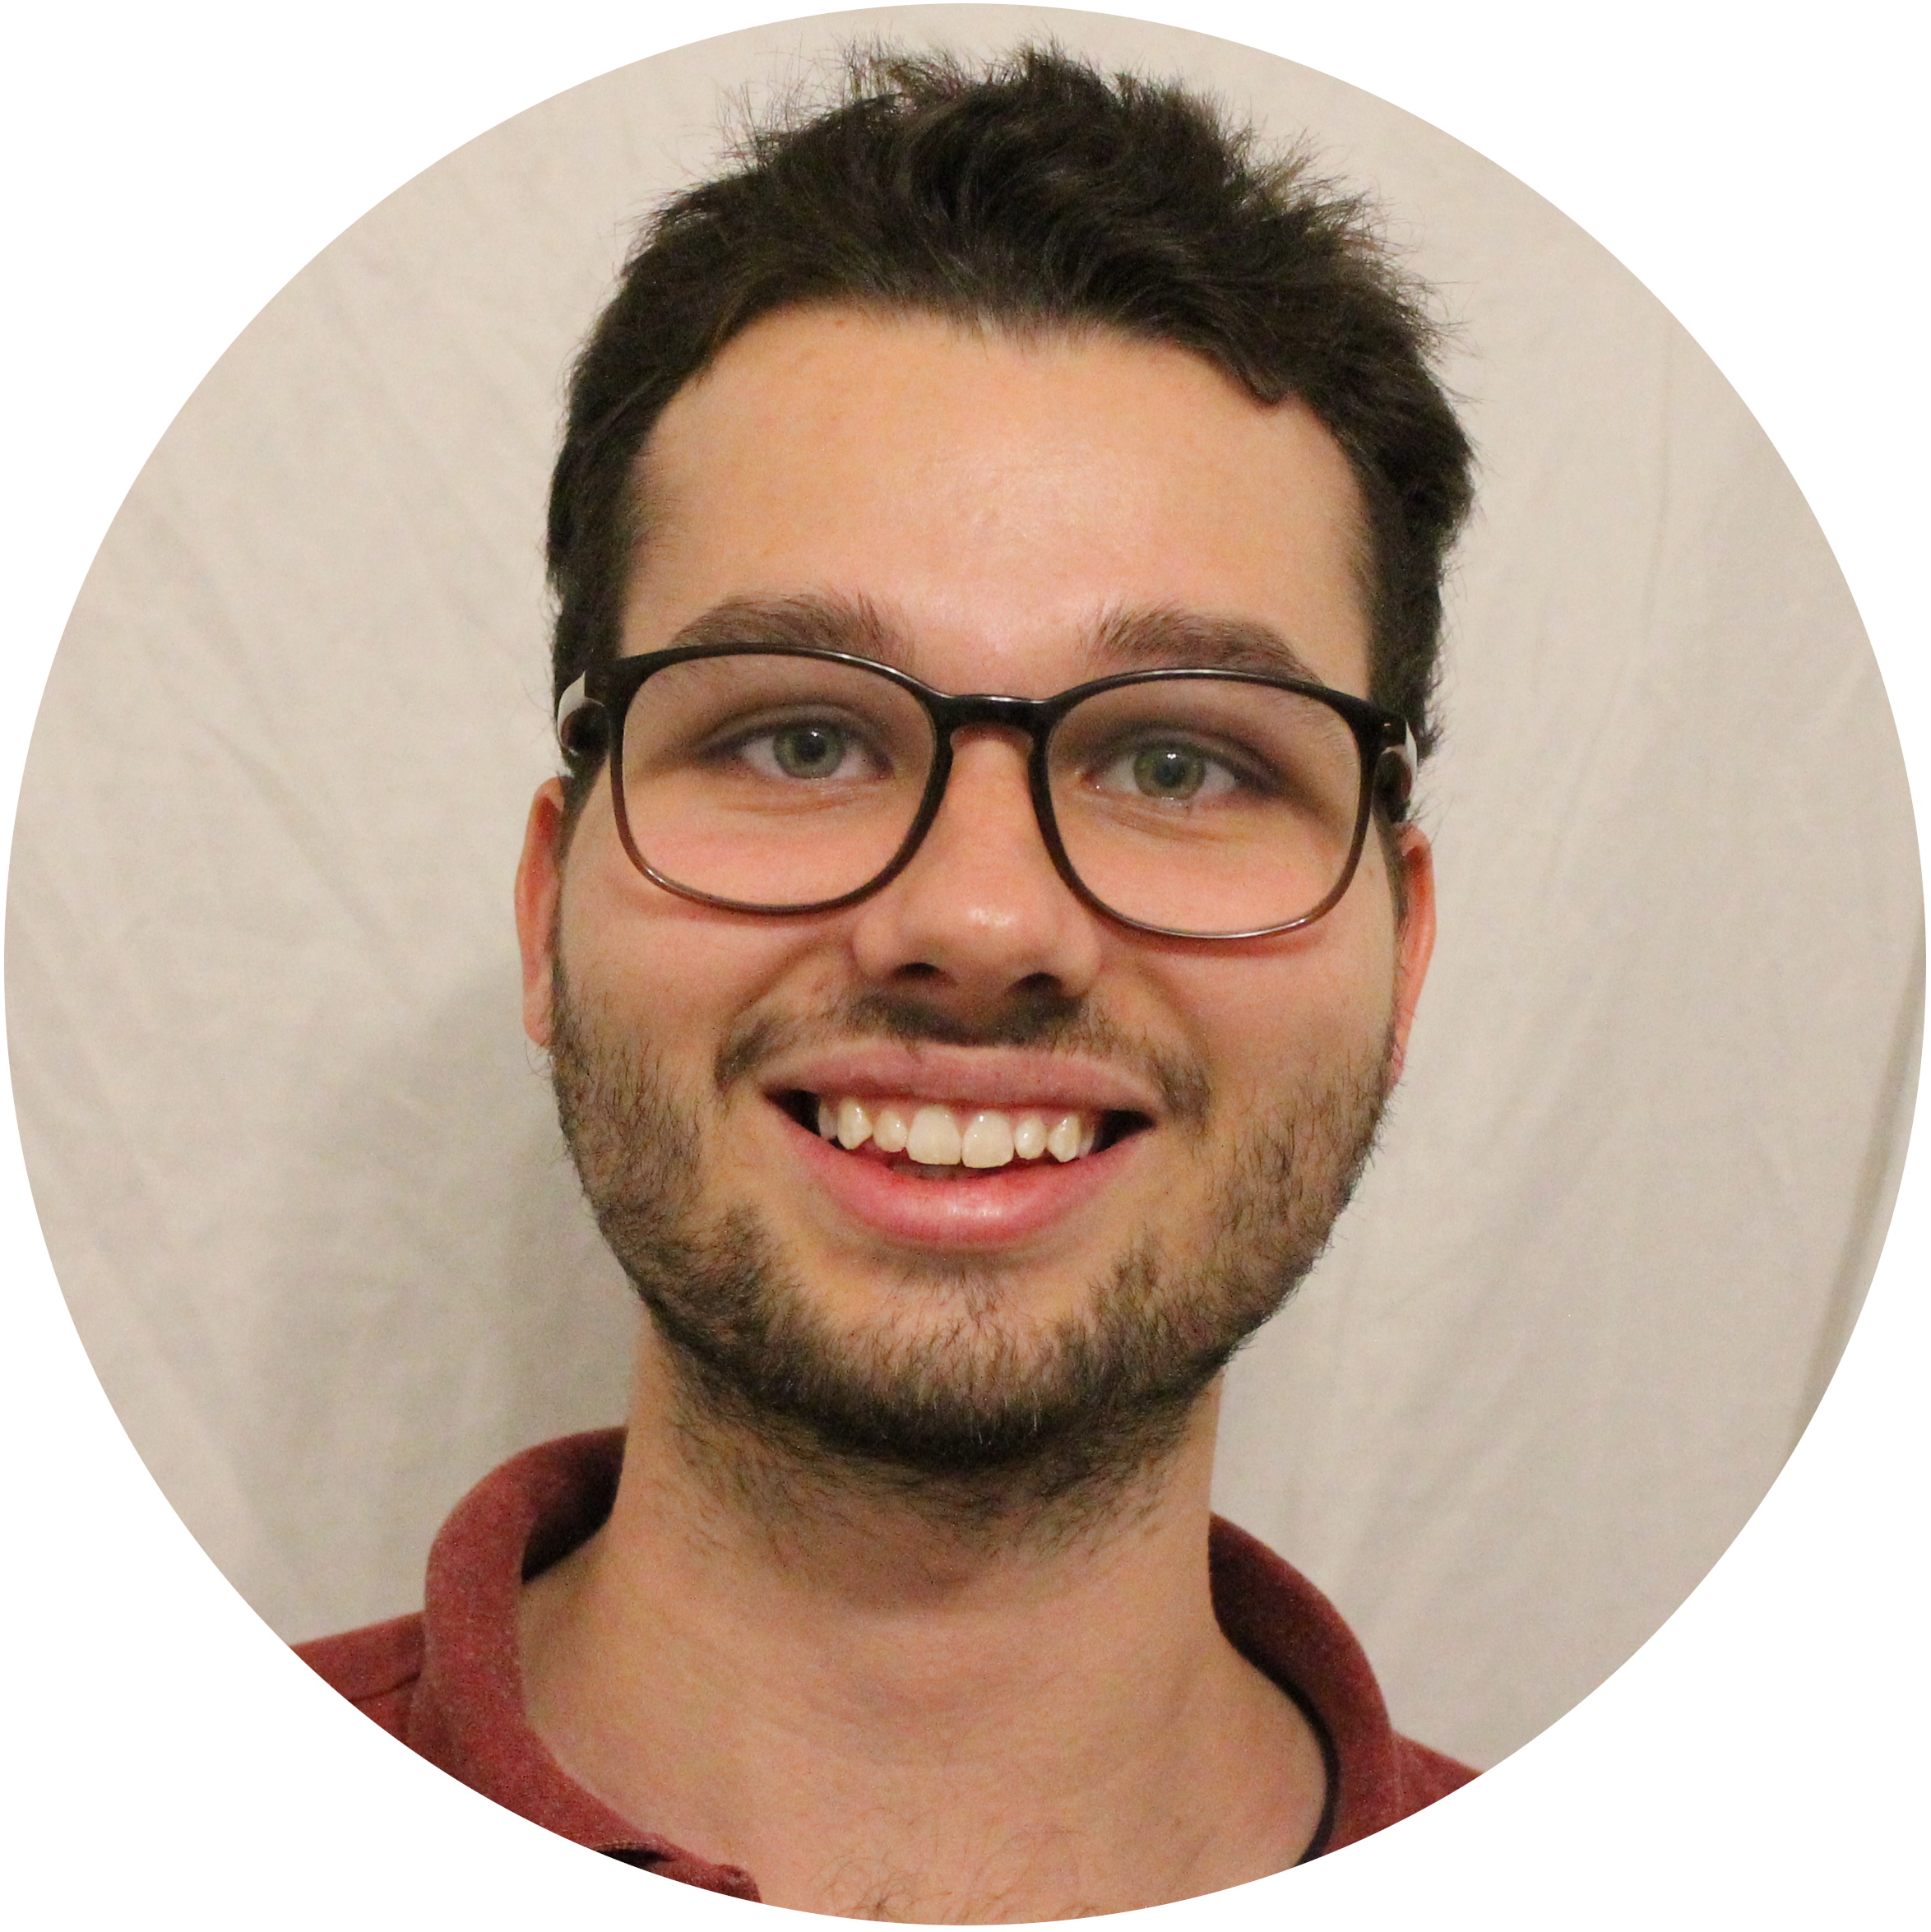
\includegraphics[scale=0.04]{img/Aaron_Circle}
\section{About Me}
~  
\textbf{nationality}
  german
   ~
  \textbf{birthplace}
  Siegen, Germany
  ~
  \textbf{birthdate}
  19.03.1996
  ~  
  \textbf{civil status}
  married, 1 child
  \section{Programming}
  ~
    \smartdiagram[bubble diagram]{
        \textbf{Python},
        \textbf{C/C++\vspace{0.2cm}},
        \textbf{CUDA\vspace{0.2cm}},
        \textbf{Fortran\vspace{1.0cm}},
        \textbf{Bash\vspace{0.2cm}},
        \textbf{Other}
    }
    \textbf{github:} 
    \href{https://github.com/AaronDavidSchneider/}{@AaronDavidSchneider}
     \section{Languages}
	  ~
    \textbf{german}
    first language
    ~
    \textbf{english}
    fluent
 \section{Interests}
~
 hiking
 singing
  %road cycling
   programming
\end{aside}

\section{Education}
\begin{entrylist}
  \entry
    {09/06-06/14}
    {Highschool}
    {Evangelisches Gymnasium Siegen-Weidenau}
    {\begin{itemize}\vspace{-3mm}
		\item advanced courses: physics, math
		\item A-level: Grade 1.6 (UK: A)
	\end{itemize}}
  \entry
    {10/15-08/18}
    {Bachelor in Physics}
    {Universität Heidelberg}
    {\begin{itemize}\vspace{-3mm}
    	\item grade: 2.0 (UK: B)
    	\item specialization: astrophysics and computational physics
    	\item bachelor thesis: Surface waves in protoplanetary disks induced by outbursts
    	\item supervisor of thesis: Prof. Dr. Cornelis P. Dullemond
    \end{itemize}
	}
  \entry
    {10/18-10/20}
    {Master in Physics}
    {Universität Heidelberg and Max Planck Institute for Astronomy}
    {\begin{itemize}\vspace{-3mm}
    	\item grade: $~$1.5 (UK: A)
    	\item specialization: Machine Learning and GPU Computing
    	\item core courses: astronomical techniques, general relativity, theoretical astrophysics, cosmology, environomental physics
    	\item master thesis: chemical composition of gas giants probed by accretion
    	\item supervisor of thesis: Dr. Bertram Bitsch
    \end{itemize}
    }
  \entry    
    {11/20-12/23}
    {Doctor of Science: Astronomy}
    {K{\o}benhavns Universitet and KULeuven}
    {\begin{itemize}\vspace{-3mm}
    \item title: Connecting the atmosphere with the interior in hot giant exoplanets
    \item Horizon 2020, Marie Sklodowska-Curie grant No 860470 (Chameleon)
    \item double degree program with Leuven and København
    \item supervisors: Dr. Ludmila Carone, Prof. Dr. Uffe Gråe Jørgensen, Prof. Dr. Leen Decin
    \end{itemize}    
	}
	\\
\end{entrylist}

\section{Softwaredevelopment (Code Owner)}
\begin{entrylist}
  \entry
    {2019-2021}
    {\texttt{SonosAlarm} (Python)}
    {\href{https://github.com/AaronDavidSchneider/SonosAlarm}{Link to Github}}
    {\texttt{HomeAssistant} component for controlling the alarm of Sonos devices. Part of the main integration since 2021. Used by 14.4\% of active \texttt{HomeAssistant} installations.}   
  \entry
    {2019-2021}
    {\texttt{ha-fritzbox-tools} (Python)}
    {\href{https://www.home-assistant.io/integrations/fritz/}{Link to Documentation}}
    {\texttt{HomeAssistant} component for controlling a Fritzbox. Part of \texttt{HomeAssistant} since 2021. Used by 7\% of active \texttt{HomeAssistant} installations.}       
  \entry
    {2020-2021}
    {\texttt{chemcomp} (Python)}
    {\href{https://chemcomp.readthedocs.io/en/latest/}{Link to Documentation}}
    {Global planetformation model, used in more than 11 publications.}    
  \entry
    {2021-2023}
    {\texttt{expeRT/MITgcm} (Fortran, Python)}
    {\href{https://exorad.readthedocs.io/en/latest/}{Link to Documentation}}
    {Accurate and efficient radiative transfer for hot Jupiters in the 3D climate model \texttt{MITgcm}, used in more than 7 publications.}   
  \entry
    {2022}
    {\texttt{bibmanager/Raycast} (Typescript, React, Python)}
    {\href{https://www.raycast.com/aaronschneider/bibmanager}{Link to Raycast store}}
    {Raycast extension for the literature management system \texttt{bibmanager}.}          
  \entry
    {2022-2023}
    {\texttt{gcm-toolkit} (Python)}
    {\href{https://gcm-toolkit.readthedocs.io/en/latest/}{Link to Documentation}}
    {Postprocessing library for reading, regridding and plotting raw GCM outputs.}          
  \entry
    {2022-2023}
    {\texttt{opacmixer} (Python)}
    {\href{https://opacmixer.readthedocs.io/en/latest/}{Link to Documentation}}
    {Machine learning framework for the accurate and efficient emulation of opacities in climate models (GCMs) or other radiative hydrodynamical applications.}      
\end{entrylist}

\newpage
\section{Fist-Author Refereed Publications}
\begin{entrylist}
  \entry
    {09/18}
    {Schneider, A. D.; Dullemond, C. P.; Bitsch, B.}
    {\href{https://arxiv.org/abs/1809.02834}{A \& A, Volume 617, id.L7}}
    {Surface waves in protoplanetary disks induced by outbursts: Concentric rings in scattered light}
  \entry
    {08/21}
    {Schneider, A. D. and Bitsch, B.}
    {\href{https://arxiv.org/abs/2105.13267}{A \& A, Volume 654, id.A71}}
    {How drifting and evaporating pebbles shape giant planets I: Heavy element content and atmospheric C/O}
  \entry
    {10/21}
    {Schneider, A. D. and Bitsch, B.}
    {\href{https://arxiv.org/abs/2109.03589}{A \& A, Volume 654, id.A72}}
    {How drifting and evaporating pebbles shape giant planets II: volatiles and refractories in atmospheres}
  \entry
    {02/22}
    {Schneider, A. D.; Carone L.; Decin L.; Jørgensen, U.G.; Mollière, P.; Baeyens, R.; Kiefer, S.; Helling, C.}
    {\href{https://arxiv.org/abs/2202.09183}{A \& A, Volume 664, id.A56}}
    {Exploring the deep atmospheres of HD 209458b and WASP-43b using a non-gray general circulation model}    
  \entry
    {10/22}
    {Schneider, A. D.; Carone L.; Decin L.; Jørgensen, U.G.; Helling, C.}
    {\href{https://arxiv.org/abs/2210.01466}{A \& A, Volume 666, id.L11}}
    {No evidence for radius inflation in hot Jupiters from vertical advection of heat}    
  \entry
  	{12/23}
    {Schneider, A. D.; Molli\`ere, P.; Louppe, G.; Carone, L.; J{\o}rgensen, U. G.; Decin, L.; Helling, C.}
    {\href{https://arxiv.org/abs/2311.00775}{A \& A, Forthcoming article}}
    {Harnessing machine learning for accurate treatment of overlapping opacity species in general circulation models}  
\end{entrylist}

\section{Other Refereed Publications}
\begin{entrylist}
  \entry
    {05/21}
    {Bitsch, B; Raymond, S. N.; Buchhave, L. A.; Bello-Arufe, A.; Rathcke, A. D.; Schneider, A. D.}
    {\href{https://arxiv.org/abs/2104.11631}{A \& A, Volume 649, id.L5}}
    {Dry or water world? How the water contents of inner sub-Neptunes constrain giant planet formation and the location of the water ice line}
  \entry
    {03/22}
    {Mollière, P.; Molyarova, T.; Bitsch, B.; Henning, T.; Schneider, A.D.; Kreidberg, L.; Eistrup, C.; Burn, R.; Nasedkin, E.; Semenov, D.; Mordasini, C.; Schlecker, M.; Schwarz, K. R.; Lacour, S.; Nowak, M.; Schulik, M.}
    {\href{https://arxiv.org/abs/2204.13714}{The Astrophysical Journal, Volume 934, Issue 1, id.74}}
    {Interpreting the atmospheric composition of exoplanets: sensitivity to planet formation assumptions}
  \entry
  	{09/22}
  	{Bitsch, B.; Schneider, A. D.; Kreidberg, L.}
  	{\href{https://arxiv.org/abs/2207.06077}{A \& A, Volume 665, id.A138}}
  	{How drifting and evaporating pebbles shape giant planets. III. The formation of WASP-77A b and \(\tau \) Boötis b}
  \entry
  	{01/23}
  	{{Samra}, D.; {Helling}, C.; {Chubb}, K. L.; {Min}, M.; {Carone}, L.; {Schneider}, A. D.}
  	{\href{https://arxiv.org/abs/2211.00633}{A \& A, Volume 669, id.A142}}
  	{Clouds form on the hot Saturn JWST ERO target WASP-96b}	
  \entry
  	{06/23}
  	{{Sainsbury-Martinez}, F.; {Tremblin}, P.; {Schneider}, A. D.; {Carone}, L.; {Baraffe}, I.; {Chabrier}, G.; {Helling}, C.; {Decin}, L.; {J{\o}rgensen}, U. G.}
  	{\href{https://arxiv.org/abs/2306.12352}{MNRAS, Volume 524, 1316–1325}}
  	{Evidence of Radius Inflation in Radiative GCM Models of WASP-76b due to the Advection of Potential Temperature}
  \entry
  	{09/23}
  	{{Chatziastros}, L.; {Bitsch}, B.; {Schneider}, A. D.}
  	{\href{https://arxiv.org/abs/2310.12797}{A \& A, Forthcoming article}}
  	{Constraining the formation history of the HAT-P-11 system by atmospheric abundances}
\end{entrylist}
\newpage
\section{Experience}
\begin{entrylist}
	\entry
    {09/14-06/15}
    {Year abroad}
    {Carnforth}
    {Theology studies}
	\entry
    {2016-2019}
    {Private tuition}
    {Heidelberg}
    {Highschool math and physics}
    \entry
    {2020}
    {Tuition}
    {Heidelberg}
    {Tuition of Introduction to Astronomy \& Astrophysics II}
    \entry
    {2023}
    {Art project}
    {K{\o}benhavn}
    {Computing the analemma for a sculpture made by danish artist Bj{\o}rn N{\o}rregard}

\end{entrylist}
\section{Volunteer Engagement}
\begin{entrylist}
  \entry
    {2015-2019}
    {voluntary work at a christian university group}
    {Heidelberg}
    {Hochschul SMD Heidelberg}
  \entry
    {2022-}
    {sound engineering}
    {K{\o}benhavn}
    {local church}    
\end{entrylist}

% Note: If space, add this:
%\vspace{1.3cm}
%\begin{flushright}
%
\includegraphics[width=.2\textwidth]{img/signature}\\
%\emph{Aaron David Schneider, \today}
%\end{flushright}
%\clearpage

%\section{Publications}
%Author, Author, Author\\
%\textbf{Lorem ipsum dolor sit amet, consectetur adipiscing elit, sed do eiusmod tempor incididunt ut labore et dolore magna aliqua}\\
%\emph{Lorem ipsum dolor sit amet, consectetur adipiscing elit, sed do eiusmod tempor incididunt ut labore et dolore magna aliqua}
%\\
%\section{Honors \& Awards}
%\begin{entrylist}
%  \entry
%    {10/2015}
%    {Best swordsman duel}
%    {Contest}
%    {Lorem ipsum.\\
%    \emph{Lorem ipsum}}
%\end{entrylist}
%
%\section{Certifications}
%\begin{entrylist}
%  \entry
%    {02/2013}
%    {Intro to Computer Science}
%    {Udacity. E-learning}
%    {\emph{Building a Python Search Engine}}
%\end{entrylist}
%
%\section{Other Info}
%For the Italian job market:\\
%\emph{Si autorizza il trattamento delle informazioni contenute nel curriculum in conformità alle disposizioni previste dal d.lgs. 196/2003. Si dichiara altresì di essere consapevole che, in caso di dichiarazioni non veritiere, si è passibili di sanzioni penali ai sensi del DPR 445/00 oltre alla revoca dei benefici eventualmente percepiti.}
%\\
%\begin{flushleft}
%\emph{May 8th, 2016}
%\end{flushleft}
%\begin{flushright}
%\emph{John Snow}
%\end{flushright}
\end{document}
